% !TEX root = ../thesis.tex
% appendix Senor Array Simulation
% @author Tobias Wulf
%

\chapter{Sensor-Array-Simulation Implementierung}\label{ch:sensor-array-sim-imp}


Der Anhang veranschaulicht die Handhabung und Standardparametrierung für die Sensor-Array-Simulation. Es sind optimale Simulationsparameter in \autoref{tab:sensor-array-sim-params} aufgeführt. Diese sind im Konfigurationsskript einzustellen und vorab der Simulation auszuführen. Das Skript erstellt eine MAT-Datei. Diese enthält, die in Gruppen zusammengefasste Simulationsparametrierung. Bei Simulationsausführung sind betreffende Parametergruppen aus der Konfigurationsdatei zu laden.


\vspace{5mm}
\begin{table}[!htbp]
	\centering
	\resizebox{\textwidth}{!}{
	\begin{tabular}{l l c c l}
		\toprule
		\textbf{Parametergruppe}                 & \textbf{Parameter} & \textbf{Wert}      & \textbf{Einheit}                & \textbf{Kurzbeschreibung}                       \\ \midrule
		\multirow{6}{*}{SensorArrayOptions}      & geometry           & 'square'           & -                               & Array-Geometrie-Indikator                       \\
		                                         & dimension          & $8$                & -                               & Sensor-Array-Pixel $N_{Pixel} \times N_{Pixel}$ \\
		                                         & edge               & $2$                & $\SI{}{\milli\metre}$           & Sensor-Array-Kantenlänge                        \\
		                                         & $V_{cc}$           & $5$                & $\SI{}{\volt}$                  & Sensor-Array-Betriebsspannung                   \\
		                                         & $V_{off}$          & $2,5$              & $\SI{}{\volt}$                  & Sensor-Brücken-Offset-Spannung                  \\
		                                         & $V_{norm}$         & $1 \cdot 10^3$     & $\SI{}{\milli\volt}$            & Kennfeldnormierung                              \\ \hline
		\multirow{4}{*}{DipoleOptions}           & sphereRadius       & $2$                & $\SI{}{\milli\metre}$           & Kugelmagnetradius                               \\
		                                         & $H_{0mag}$         & $200$              & $\SI{}{\kilo\ampere\per\metre}$ & Betragsfeldstärke Magnetfeldnormierung          \\
		                                         & $z_0$              & $1$                & $\SI{}{\milli\metre}$           & $Z$-Abstand Magnetfeldnormierung                \\
		                                         & $m_{0mag}$         & $1 \cdot 10^6$     & $\SI{}{\ampere\square\metre}$   & Magnitude d. mag. Moments                       \\ \hline
		\multirow{10}{*}{Training-/ TestOptions} & useCase            & 'Training'/ 'Test' & 'char'                          & Datensatzindikator f. Anwendungszweck           \\
		                                         & xPos               & $\left[0,\right]$  & $\SI{}{mm}$                     & Sensor-Array $X$-Positionsvektor                \\
		                                         & yPos               & $\left[0,\right]$  & $\SI{}{mm}$                     & Sensor-Array $Y$-Positionsvektor                \\
		                                         & zPos               & $\left[7,\right]$  & $\SI{}{mm}$                     & Sensor-Array $Z$-Positionsvektor                \\
		                                         & tilt               & $0$                & $\SI{}{\degree}$                & Magnetverkippung in $Y$-Achse                   \\
		                                         & angleRes           & $0,5$              & $\SI{}{\degree}$                & Winkelauflösung f. Magnetrotation               \\
		                                         & phaseIndex         & 0                  & -                               & Phasenverschiebung-Index f. Startwinkel         \\
		                                         & nAngles            & $20$/ $720$        & -                               & Anzahl gleich verteilter Simulationswinkel      \\
		                                         & BaseReference      & 'TDK'              & char                            & Kennfelddatensatzindikator                      \\
		                                         & BridgeReference    & 'Rise'             & char                            & Kennfeldindikator                               \\ \bottomrule
	\end{tabular}}
	\caption[Sensor-Array-Simulationsparameter]{Sensor-Array-Simulationsparameter. Default-Parameter für die Simulation mit ideal ausgerichteten Gesamtsystem, bestehend aus mag. Dipol und Sensor-Array.}
	\label{tab:sensor-array-sim-params}
\end{table}


\clearpage


Die Sensor-Array-Simulation folgt der Aufführung in \autoref{alg:sensor-array-sim}. Zur Generierung von Trainings-/ Testdatensätze dient die Konfigurationsdatei als Eingabe. Entsprechend der Parametrierung in \autoref{tab:sensor-array-sim-params}, sind notwendige Kennfelddatensätze initialisiert und Funktionsmodule eingebunden. Für die eingestellte Anzahl von Simulationswinkeln und angegebenen Winkelauflösung, wird ein Rotationsvektor aufgestellt, indem alle Simulationswinkel gleich verteilt sind. Die Simulation fährt alle $X,Y,Z$ Sensor-Array-Positionen im Koordinatenraum ab. Für jede angefahrene Position wird ein Meshgrid und entsprechender Datensatz mit voller Rotation erzeugt. Für verschiedene Magnetverkippung ist die Konfigurationsdatei anzupassen und die Simulation zu wiederholen.


\begin{algorithm}[hbp]
	\SetAlgoLined
	\KwIn{Konfigurationsdatensatz}
	\KwOut{MAT-Dateipfad}
	\KwResult{Sensor-Array-Datensätze (Training/ Test)}
	\textbf{1.} Laden der Konfigurierung $\leftarrow$ \autoref{tab:sensor-array-sim-params}\;
	\textbf{2.} Laden der Kennfelder $\leftarrow$ \autoref{ch:tdk-datensatz}\;
	\textbf{3.} Initialisierung Simulationsparameter $\leftarrow$ \autoref{tab:sensor-array-sim-params}\;
	\textbf{4.} Initialisierung Rotation $\leftarrow$ \autoref{eq:ruhepos}, \autoref{eq:ruhemom}\;
	\textbf{5.} Initialisierung Kennfelder $\leftarrow$ \autoref{eq:vout-tdk}\;
	\textbf{6.} Initialisierung Dipol-Rotationsmomente $\leftarrow$ \autoref{eq:allgrot}\;
	\textbf{7.} Initialisierung Sensor-Array-Positionen $\leftarrow$ \autoref{tab:sensor-array-sim-params}\;
	\textbf{8.} Initialisierung Dipol-Feldnormierung $\leftarrow$ Betragskonstante in \autoref{eq:dipnorm}\;
	\textbf{10.} Speicherallokation f. Ergebnisse\;
	\textbf{11.} Anlegen Metadaten (Info) und Simulationsdaten (Data) Structs\;
	\textbf{12.} \For{$z$ in $Z$-Positionsvektor}{
		\For{$x$ in $X$-Positionsvektor}{
			\For{$y$ in $Y$-Positionsvektor}{
				Update Info-Struct (Positionsdaten)\;
				Initialisierung Sensor-Array-Meshgrid $\leftarrow$ \autoref{eq:arraymeshgrid}\;
				\For{$\vec{m}_i$ in Momentenmatrix}{
					Normierte Dipol-Feldberechnung auf Meshgrid $\leftarrow$ \autoref{eq:dipnorm}\;
					Kennfeld-Mapping interp2(Nearest-Neighbor) $\leftarrow$ \autoref{fig:kennfeld-mapping}\;
				}
				Update Data-Struct (Ergebnisse)\;
				Speichern Info- und Data-Struct in Ziel-MAT-Datei\;
				Ausgabe MAT-Dateipfad\;
			}
		}
	}
	\caption{Sensor-Array-Simulation}
	\label{alg:sensor-array-sim}
\end{algorithm}


\clearpage


\begin{figure}[tph]
	\centering
	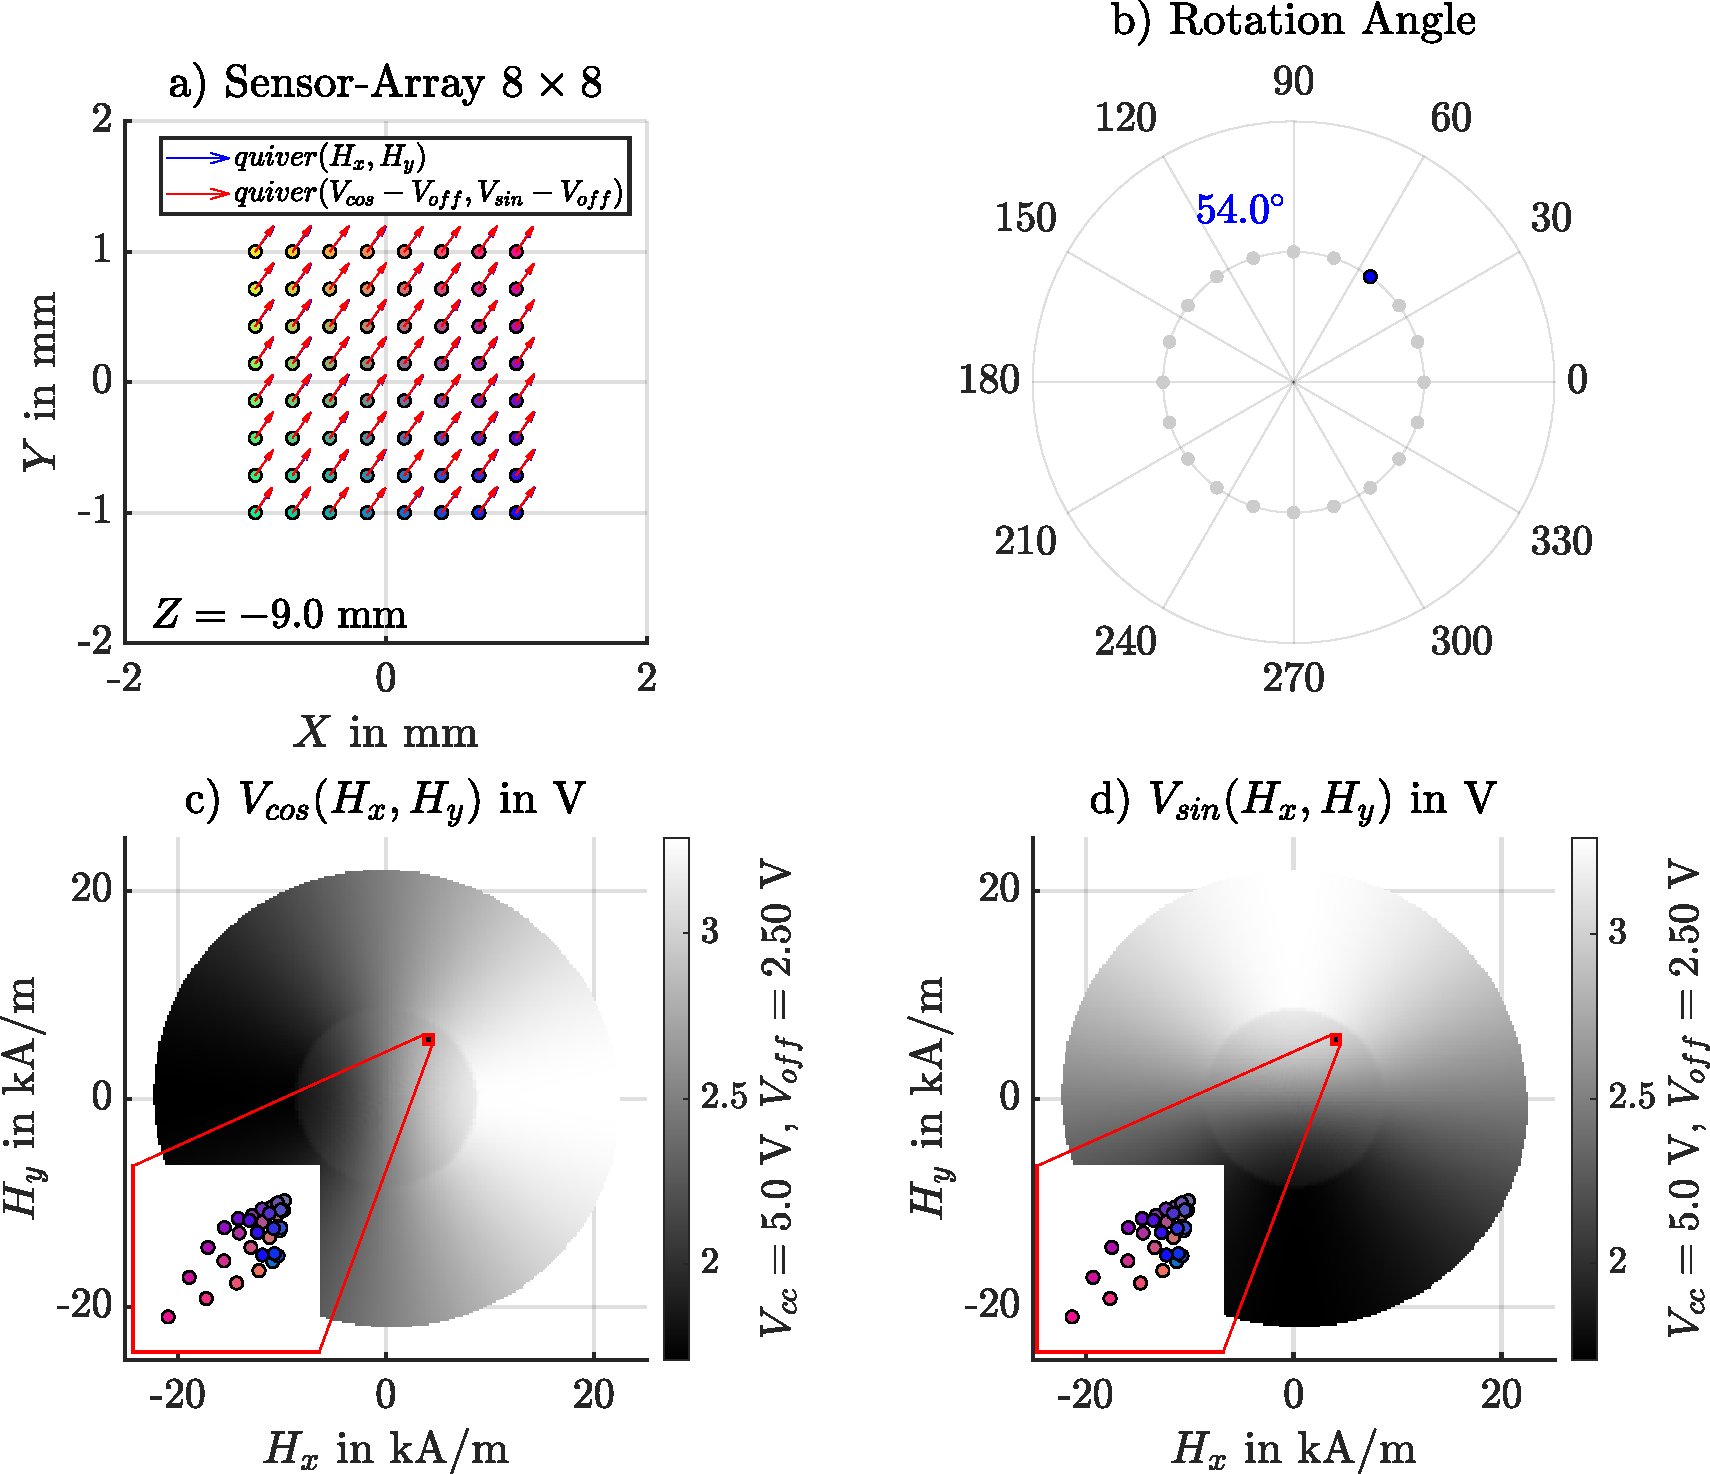
\includegraphics[width=.99\linewidth]{appendix/images/5-Sensor-Array-Sim-Imp/Kennfeld-Mapping}
	\caption[Kennfeld-Mapping]{Kennfeld-Mapping. Entnahme von Referenzspannungen aus Sensor-Kennfelder, gezeigt für einen beliebigen Simulationswinkel. In a) Meshgrid des Sensor-Arrays mit Grundposition $(0,0,-9)^T \SI{}{\milli\metre}$ relativ zum Koordinatenursprung (mag. Dipol). Simulation ohne Dipol-Verkippung. b) Simulation für $20$ gleich verteilte Winkel, gezeigt ist der vierte Winkel bei $\SI{54}{\degree}$. Simulationsparameter sind wie in \autoref{tab:sensor-array-sim-params} eingestellt. Magnet und Array-Position sind ideal konfiguriert. Ersichtlich anhand des eng gegliederten Feldstärken-Mappings auf c) Cosinus-Kennfeld und d) Sinus-Kennfeld. Die simulierten Feldstärken für alle Sensor-Pixel-Koordinaten, liegen innerhalb des linearen Kennfeldarbeitsbereich. Die Kennfelder sind entsprechend Betriebsspannungsparametrierung in $\SI{}{\volt}$ umgerechnet.}
	\label{fig:kennfeld-mapping}
\end{figure}


\clearpage


\autoref{fig:kennfeld-mapping} zeigt das Mapping, auf TMR-Sensor-Kennfeldern (\autoref{ch:tdk-datensatz}), für prozessierte $H_x$- und $H_y$-Feldstärken. Die Simulation ist mit der Standardparametrierung aus \autoref{tab:sensor-array-sim-params} ausgeführt worden. Hier am Beispiel für $20$ Simulationswinkel. Gezeigt ist der vierte Winkel bei $\SI{54}{\degree}$. Die errechneten Feldstärken sind auf die Kennfelder projiziert und Spannungswerte mittels Matlab-2D-Interpolation für Nearest-Neighbor entnommen. \autoref{fig:senor-array-teilansicht} zeigt, das nochmals für $720$ Winkel und vier Sensor-Pixel. Es sind die Eck-Pixel angezeigt. Da sich der mag. Dipol ohne Verkippung, zentriert über dem Sensor-Array befindet, überlagern sich die Signalverläufe für diagonal gegenüberliegende Sensor-Pixel. Die leicht ellipsenförmige Verlauf der projizierten Feldstärken, der äußeren Pixel, ergibt sich durch den Versatz zur Magnetfeldmitte. Ein Pixel direkt lotrecht zur Magnet-$Z$-Achse platziert, erzeugt einen optimale Kreisbahn. Eine detaillierte Beschreibung des Funktionsmoduls ist in \autoref{mcode:sensorarraysimulation} einzusehen.


\vspace{4mm}
\begin{figure}[bph]
	\centering
	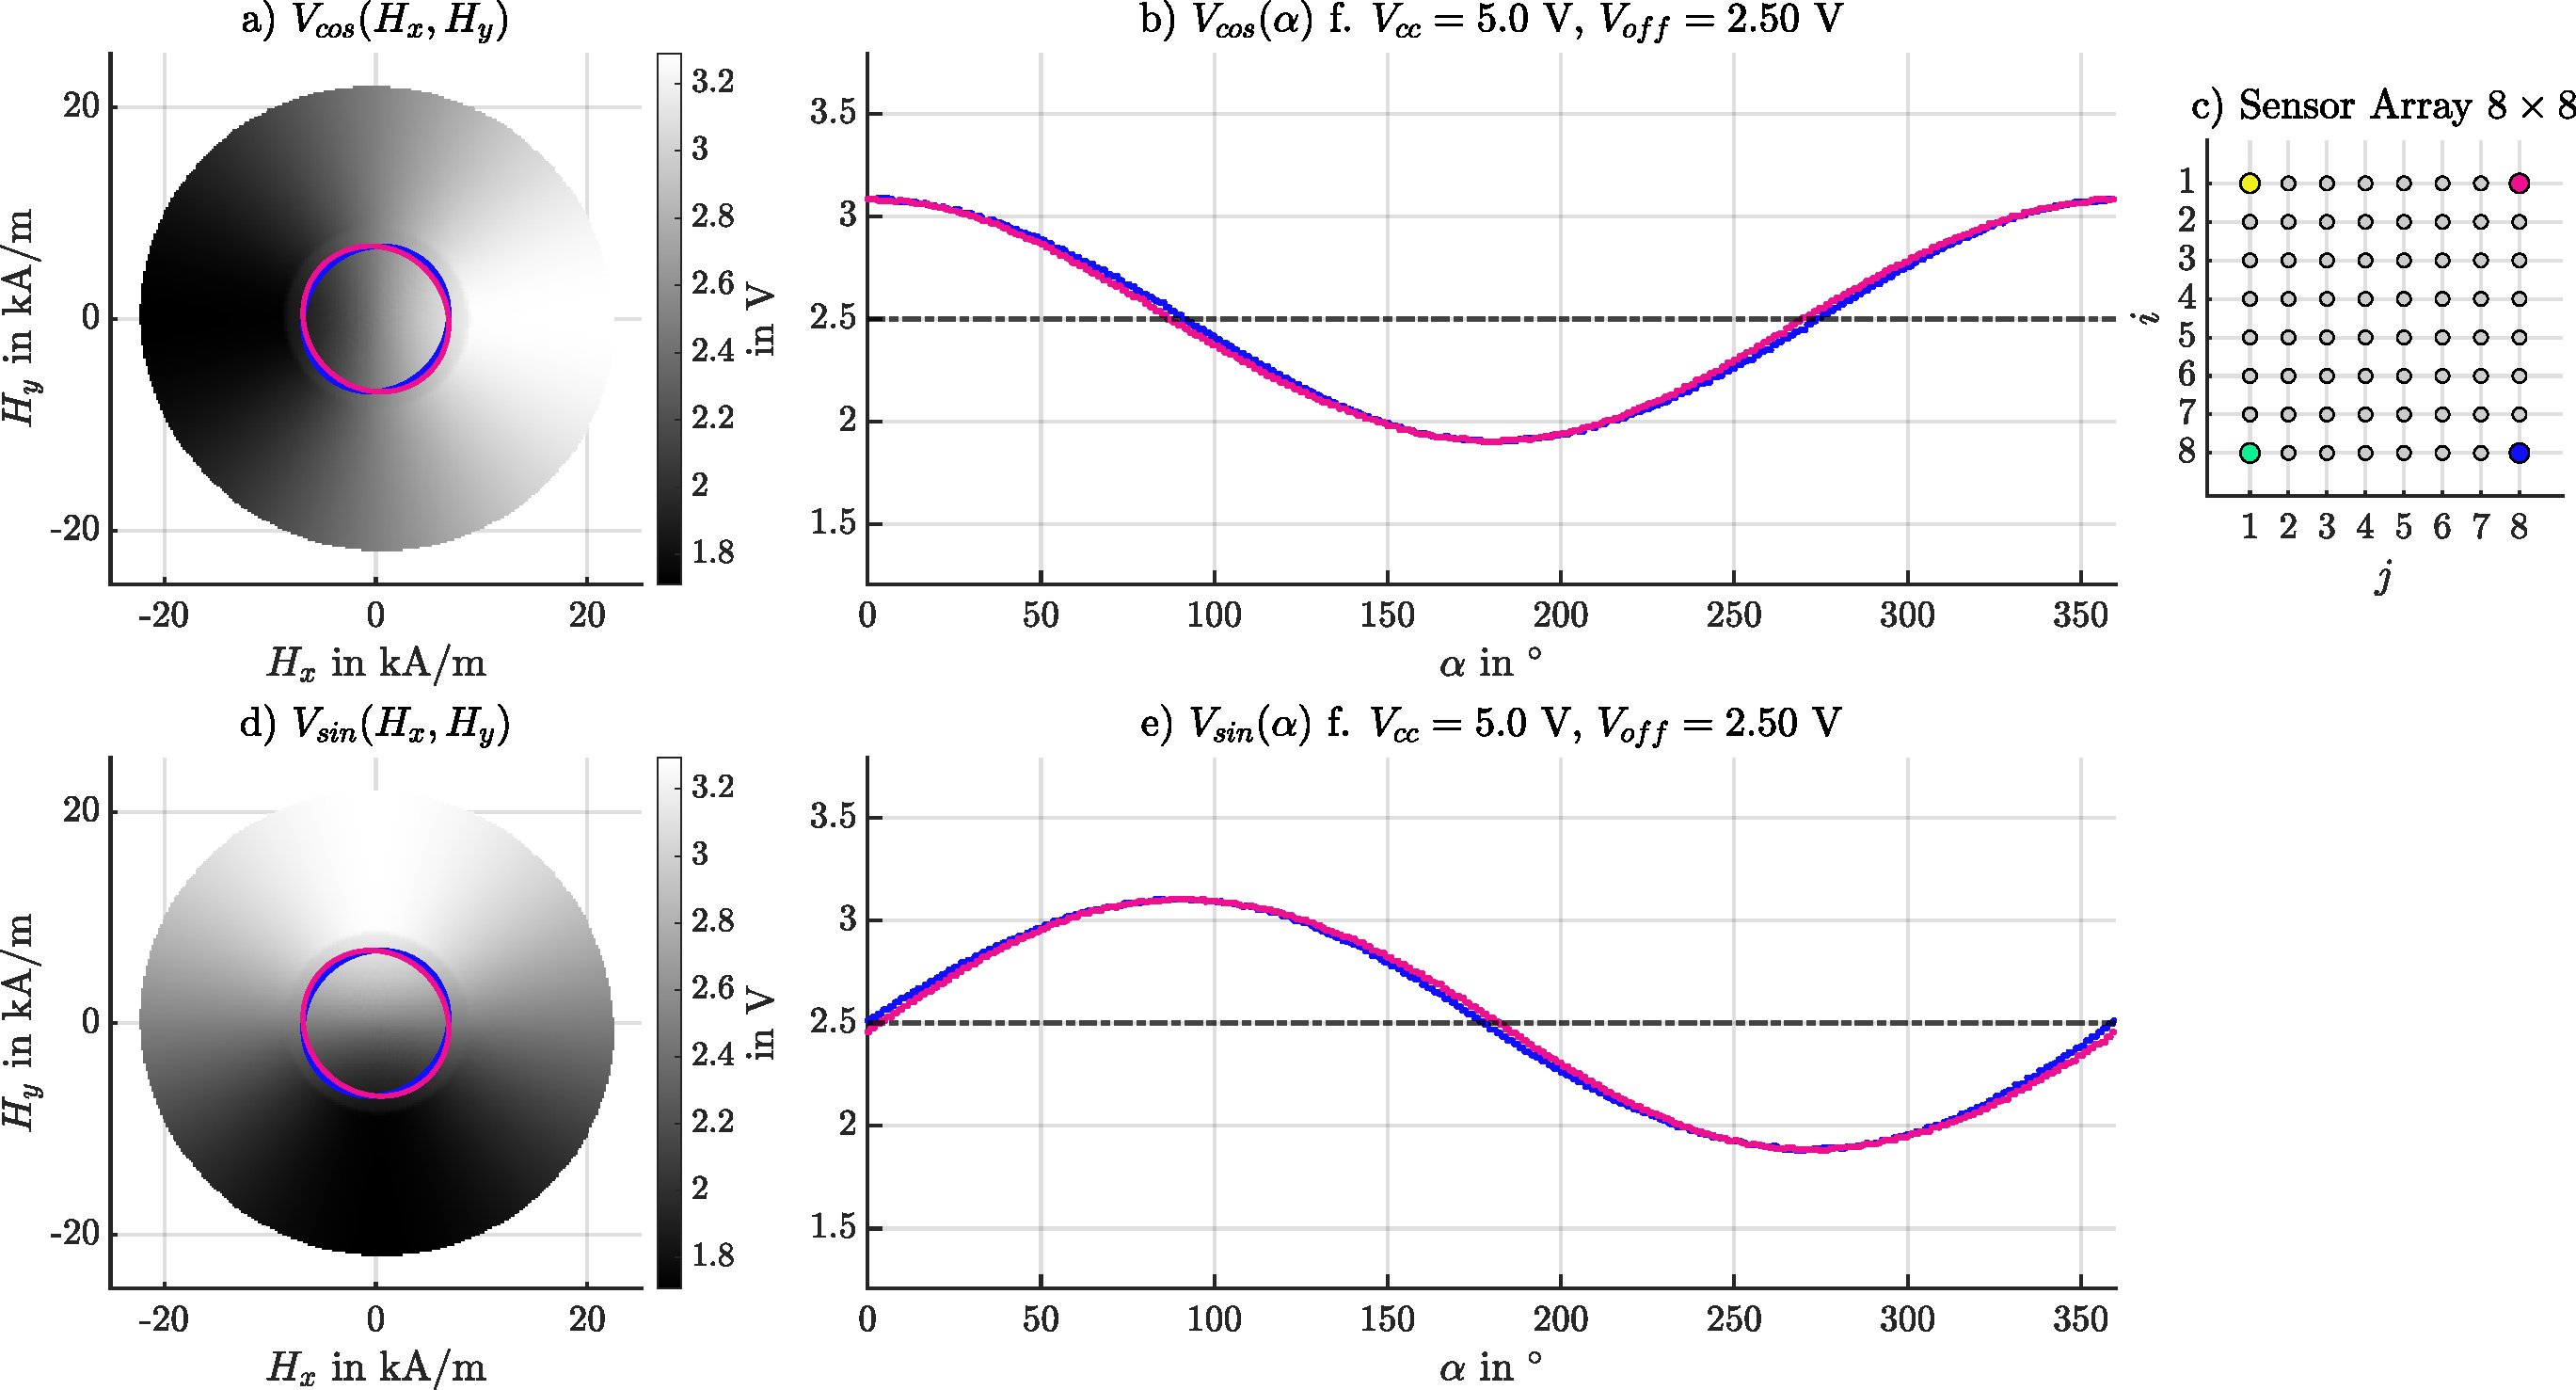
\includegraphics[width=\linewidth]{appendix/images/5-Sensor-Array-Sim-Imp/Senor-Array-Teilansicht}
	\caption[Sensor-Array-Datensatz Teilansicht]{Sensor-Array-Datensatz Teilansicht. Teilansicht der Simulationsergebnisse, entsprechend der Parametrierung nach \autoref{tab:sensor-array-sim-params}. Es ist der gesamte Simulationsdurchlauf für die Eck-Sensor-Pixel c) gezeigt. a) und d) zeigt das Kennfeld-Mapping, für korrespondierende Feldstärken, bei einer vollständigen Dipol-Drehung. b) und e) stellt die Rotation aufgetragen über alle Simulationswinkel dar. Die sich diagonal gegenüberliegenden Sensor-Pixel, überlagern sich in den Darstellungen a), b), d) und e). Das entspricht der Kreuzsymmetrieeigenschaft Dipol-Magnetfeldes. Das Sensor-Array ist zentriert zum Dipol ausgerichtet. Dipol ist nicht verkippt. Grafik nachempfunden aus \cite{Schuethe2019}}
	\label{fig:senor-array-teilansicht}
\end{figure}
